%&pdflatex --translate-file=cp1250pl

\documentclass[10pt]{article}

\usepackage[pdftex]{graphicx}
\graphicspath{{./pdf/}}

\usepackage{csagh}

% Packages I added 
\usepackage{minted}


\begin{document}
\begin{opening}

\title{Combinatory Logic}
\author[conorhoekstra@gmail.com, Toronto, ON, Canada]{Conor Hoekstra}

\begin{abstract}
  As the name suggests... an English abstract.
\end{abstract}

\keywords{...}
\begin{abstract}
An abstract goes here\ldots
	
The structure of the paper does not have to be followed, it is just
a reasonable example. If you're writing a paper for the first time, please consult:
http://cs.stanford.edu/people/widom/paper-writing.html

Note, BibTex with cs-agh.bst must be used for formatting your references!
\end{abstract}

\keywords{combinatory logic, combinators, programming languages}

\end{opening}

\section{Introduction}

Lorem ipsum dolor sit amet, consectetur adipiscing elit. Nunc suscipit lacus id tortor porta, a fermentum enim lobortis. Nullam ac risus ultricies, auctor nunc eget, tristique lacus. Nullam ante lorem, volutpat at nibh ut, gravida fringilla diam. Lorem ipsum dolor sit amet, consectetur adipiscing elit. Vestibulum viverra eleifend quam.

\section{Combinators}

\subsection{Combinator Lambda Expressions}

\begin{table}[!htb]
  \begin{tabular}{cc}
     \hline
     {\bf Combinator} & {\bf Lambda Expression} \\ 
     \hline I & $\lambda$a.a \\
     K & $\lambda$ab.a \\
     W & $\lambda$ab.abb \\
     C & $\lambda$abc.acb \\
     B & $\lambda$abc.a(bc) \\
     S & $\lambda$abc.ac(bc) \\
     D & $\lambda$abcd.ab(cd) \\
     B$_1$ & $\lambda$abcd.a(bcd) \\
     $\Psi$ & $\lambda$abcd.a(bc)(bd) \\
     $\Phi$ & $\lambda$abcd.a(bd)(cd) \\
     D$_2$ & $\lambda$abcde.a(bd)(ce) \\
     E & $\lambda$abcde.ab(cde) \\
     $\Phi_1$ & $\lambda$abcde.a(bde)(cde) \\
     Ê & $\lambda$abcdefg.a(bde)(cfg) \\
     \hline
  \end{tabular}
  \end{table}

\subsection{Combinators Across Programming Languages}

\subsubsection{Combinators in Haskell}

\begin{table}[!htb]
  \begin{tabular}{ccc}
     \hline
     {\bf } & {\bf Name} & {\bf Library} \\ 
     \hline 
     I & \mintinline{haskell}{id} & Prelude \\
     K & \mintinline{haskell}{const} & Prelude \\
     W & \mintinline{haskell}{join} & Control.Monad \\
     C & \mintinline{haskell}{flip} & Prelude \\
     B & \mintinline{haskell}{(.)} & Prelude \\
     S & \mintinline{haskell}{(<*>)} / \mintinline{haskell}{ap} & Control.Applicative \\
     B$_1$ & \mintinline{haskell}{(.:)} & Data.Composition \\
     $\Psi$ & \mintinline{haskell}{on} & Data.Function \\
     $\Phi$ & \mintinline{haskell}{liftA2} & Control.Applicative \\
     A & \mintinline{haskell}{($)} & Prelude \\
     \hline
  \end{tabular}
  \end{table}

\subsubsection{Combinators in APL}

\subsubsection{Combinators in J}

\subsubsection{Combinators in BQN}

\section{Contributions}

\subsection{Missing Combinators}

\subsection{Combinator Hierarchy}

\subsubsection{D$_2$ Family}

\subsubsection{E Family}

\subsubsection{B Family}

\subsubsection{D$_2$, E, B Families Combined}

\begin{figure}[!htb]
  \centerline{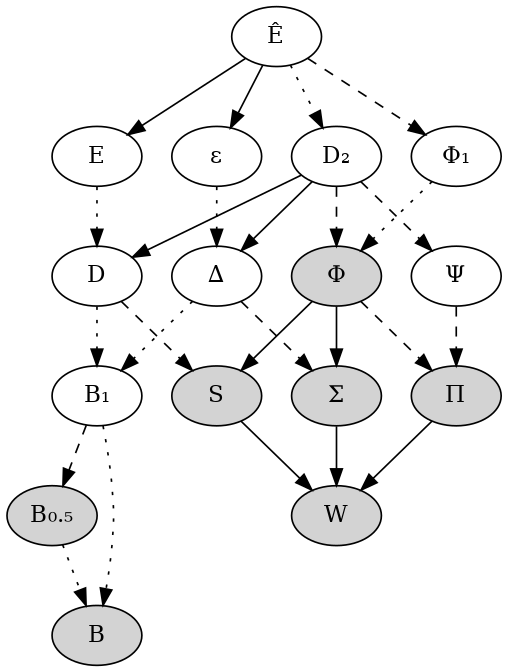
\includegraphics[scale = 0.5]{./combinator-d2-e-b-connected.png}}
  \caption{D$_2$, E, B combinator hierarchy.} % \label{fig:2}
\end{figure}

Nam fringilla, ante in varius imperdiet, metus dolor facilisis tellus, eget viverra tortor neque in massa. Vivamus eget viverra justo. Duis et bibendum eros. Etiam nibh arcu, condimentum vitae laoreet eget, vulputate sed arcu. Fusce scelerisque, ex tristique consequat blandit, nulla arcu imperdiet sem, vel scelerisque urna lorem nec elit. Nam vestibulum dui vel volutpat congue.

\begin{figure}[!ht]
\centering
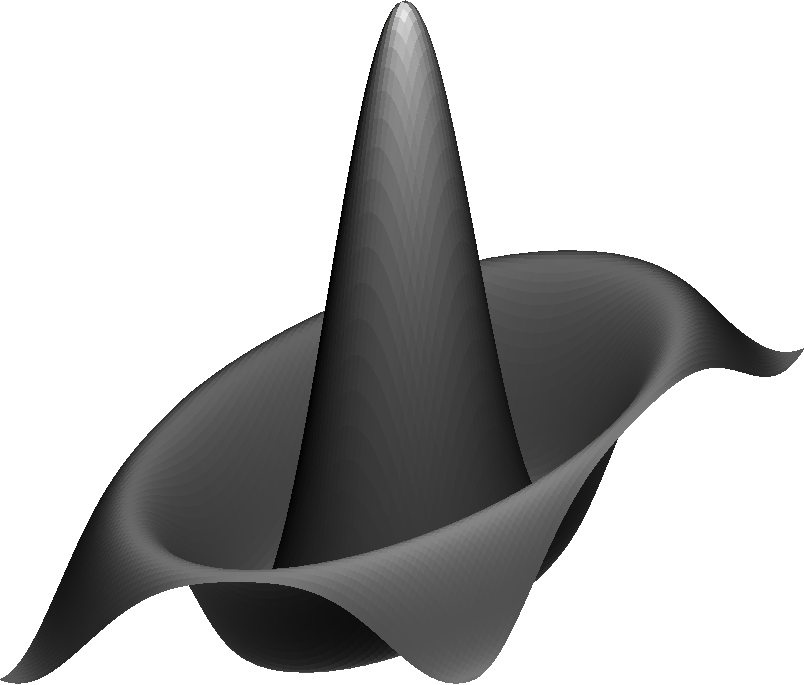
\includegraphics[scale=.4]{surfz}
\caption{An example of including the PDF graphics in the text ---
function $z=\frac{\sin(x^2+y^2)}{x^2+y^2}$}
\label{rys:surf}
\end{figure}

Nam viverra maximus tortor, sed accumsan odio iaculis et. Nulla facilisi. Aliquam eget elit massa. Nulla volutpat vel eros ac eleifend. Ut cursus, risus ac laoreet iaculis, nibh sapien mollis sem, sit amet luctus arcu nibh nec arcu. Donec sit amet nisi id quam convallis ultrices. Nullam sagittis ultrices volutpat. 

\section{Comparison/Experiments/\ldots}

Nullam ac efficitur turpis. Integer fringilla sapien sit amet luctus porta. In eu lobortis diam, at ornare tortor. Phasellus pretium est non quam ultricies, eget molestie massa rhoncus. Vivamus pulvinar tempor sem ut pulvinar. Aliquam tempus elementum dictum.

\begin{table}[!ht]
\centering
\caption{Sample table with sample data}
\label{tabl.1}
  \begin{tabular}{|l<{.}|c|>{$}c<{$}|r|}
                                 \hline
   1 & a~   & \alpha &  10\,000\\\hline
   2 & bb   & \beta  &  25\,000\\\hline
   3 & ccc  & \gamma & 100\,000\\\hline
   4 & dddd & \delta & 125\,000\\\hline
  \end{tabular}
\end{table}

Etiam gravida odio in ante venenatis, a tincidunt tortor eleifend. Phasellus sollicitudin ut ex at bibendum. Proin et laoreet dui, quis luctus ante. Praesent condimentum orci pretium ante sollicitudin, in facilisis odio iaculis. 


\section{Conclusion}

Aliquam quis libero aliquet, porttitor magna tincidunt, pellentesque lectus. Quisque a lacus tortor. Phasellus vitae mi vulputate, tincidunt urna nec, rutrum urna. In malesuada leo iaculis, tristique neque id, bibendum ipsum. Suspendisse lacus turpis, euismod sit amet neque non, ullamcorper porta ligula.

\begin{acknowledgements}
 The research presented in this paper was partially supported by \ldots
\end{acknowledgements}

\nocite{*} %REMOVE

\bibliographystyle{cs-agh}
\bibliography{bibliography}

\end{document}